%%%%%%%%%%%%%%%%%%%%%%%%%%%%%%%%%%%%%%%%%%%%%%
% GHALI CONSULTANTS - ACI 318-19 METHOD C TEMPLATE
% Two-Column Academic Format for Column Design
% Method C Slenderness Analysis per ACI 318-19
% Version 2025.1 - Academic Professional Style
%%%%%%%%%%%%%%%%%%%%%%%%%%%%%%%%%%%%%%%%%%%%%%

\documentclass[
  10pt,
  letterpaper,
  twocolumn
]{article}

% Essential packages for academic engineering documents
\usepackage[a4paper, margin=2cm, top=2.5cm, bottom=2cm, columnsep=1cm]{geometry}
\usepackage{amsmath,amsfonts,amssymb}
\usepackage[nopatch]{microtype}
\usepackage{booktabs}
\usepackage{graphicx}
\usepackage{float}
\usepackage{xcolor}
\usepackage{array}
\usepackage{tabularx}
\usepackage{longtable}
\usepackage{multirow}
\usepackage{siunitx}
\usepackage{fancyhdr}

% Font configuration - Aptos Narrow alternative (using condensed font)
\usepackage[scaled=0.92]{helvet}
\renewcommand{\familydefault}{\sfdefault}
\usepackage[T1]{fontenc}

% Define Ghali Consultants color scheme (subdued for academic)
\definecolor{ghaliblue}{RGB}{31, 78, 121}      % Professional blue
\definecolor{ghalired}{RGB}{197, 80, 75}       % Accent red  
\definecolor{ghaligreen}{RGB}{76, 175, 80}     % Success green
\definecolor{ghaligray}{RGB}{88, 88, 88}       % Text gray
\definecolor{lightgray}{RGB}{245, 245, 245}    % Table background

% Page style configuration - narrow headers/footers
\pagestyle{fancy}
\fancyhf{}
\renewcommand{\headrulewidth}{0.3pt}
\renewcommand{\footrulewidth}{0.3pt}

% Narrow headers and footers with small font
\fancyhead[L]{\scriptsize\textcolor{ghaliblue}{\textbf{Ghali Consultants}}}
\fancyhead[R]{\scriptsize\textcolor{ghaligray}{Column Design | Page \thepage}}

\fancyfoot[L]{\scriptsize\textcolor{ghaligray}{ACI 318-19 Method C}}
\fancyfoot[C]{\scriptsize\textcolor{ghaligray}{Professional Engineering}}
\fancyfoot[R]{\scriptsize\textcolor{ghaligray}{\today}}

% Title page style
\fancypagestyle{firstpage}{
  \fancyhf{}
  \renewcommand{\headrulewidth}{0pt}
  \renewcommand{\footrulewidth}{0.3pt}
  \fancyfoot[C]{\scriptsize\textcolor{ghaligray}{Ghali Consultants - Structural Engineering Services}}
  \fancyfoot[R]{\scriptsize\textcolor{ghaligray}{\today}}
}

% Section formatting - academic style
\usepackage{titlesec}
\titleformat{\section}
  {\large\bfseries\color{ghaliblue}}
  {\thesection}{0.5em}{}
\titleformat{\subsection}
  {\normalsize\bfseries\color{ghaligray}}
  {\thesubsection}{0.5em}{}
\titleformat{\subsubsection}
  {\small\bfseries\color{ghaligray}}
  {\thesubsubsection}{0.5em}{}

% Enhanced table formatting for academic style
\renewcommand{\arraystretch}{1.2}
\newcolumntype{L}[1]{>{\raggedright\arraybackslash}p{#1}}
\newcolumntype{C}[1]{>{\centering\arraybackslash}p{#1}}
\newcolumntype{R}[1]{>{\raggedleft\arraybackslash}p{#1}}

% Units formatting
\sisetup{
  per-mode=fraction,
  fraction-function=\tfrac,
  unit-color=ghaligray,
  separate-uncertainty=true
}

\begin{document}

\thispagestyle{firstpage}

% Title and author information (academic style)
\begin{center}
{\Large\textbf{\textcolor{ghaliblue}{ACI 318-19 Method C Column Design}}} \\[0.3cm]
{\large\textcolor{ghaligray}{Slenderness Analysis and Moment Magnification}} \\[0.5cm]
{\normalsize\textcolor{ghaliblue}{Ahmed Ghali, P.E.} | \textcolor{ghaligray}{Lead Structural Engineer}} \\
{\normalsize\textcolor{ghaligray}{Ghali Consultants | \today}} \\[1cm]
\end{center}

% Abstract section
\section*{\textcolor{ghaliblue}{Abstract}}
This technical report presents comprehensive analysis of reinforced concrete column design using ACI 318-19 Method C (Moment Magnification). The analysis evaluates slenderness effects, critical buckling loads, and moment magnification factors for rectangular columns subjected to combined axial load and bending. The methodology follows ACI 318-19 Section 6.6 requirements with systematic verification of stability and strength criteria.

\textbf{Keywords:} column design, slenderness, Method C, ACI 318-19, moment magnification, buckling

% Project summary table (academic style)
\section{Project Overview}

\begin{table}[h]
\centering
\caption{Project Information Summary}
\label{tab:project_info}
\begin{tabular}{@{}ll@{}}
\toprule
\textbf{Parameter} & \textbf{Value} \\
\midrule
Project ID & PROJECT_ID_PLACEHOLDER \\
Column ID & COLUMN_ID_PLACEHOLDER \\
Design Code & ACI 318-19 \\
Analysis Method & Method C (Moment Magnification) \\
Engineer & Ahmed Ghali, P.E. \\
Reviewer & Senior Engineer, P.E. \\
\bottomrule
\end{tabular}
\end{table}

\section{Design Parameters}

\subsection{Material Properties}

The material properties listed in Table~\ref{tab:materials} comply with ACI 318-19 specifications for reinforced concrete column design.

\begin{table}[h]
\centering
\caption{Material Properties}
\label{tab:materials}
\begin{tabular}{@{}lcc@{}}
\toprule
\textbf{Property} & \textbf{Value} & \textbf{Unit} \\
\midrule
Concrete Strength, $f'_c$ & FC_PRIME_PLACEHOLDER & MPa \\
Steel Yield Strength, $f_y$ & FY_PLACEHOLDER & MPa \\
Concrete Modulus, $E_c$ & EC_PLACEHOLDER & MPa \\
Steel Modulus, $E_s$ & 200,000 & MPa \\
\bottomrule
\end{tabular}
\end{table}

\subsection{Column Geometry}

Table~\ref{tab:geometry} summarizes the geometric properties of the analyzed column, with critical buckling direction identified.

\begin{table}[h]
\centering
\caption{Column Geometry}
\label{tab:geometry}
\begin{tabular}{@{}lcc@{}}
\toprule
\textbf{Parameter} & \textbf{Value} & \textbf{Unit} \\
\midrule
Width (short), $b$ & B_PLACEHOLDER & mm \\
Height (long), $h$ & H_PLACEHOLDER & mm \\
Unsupported Length, $L_u$ & LU_PLACEHOLDER & mm \\
Effective Length, $L_e$ & LE_PLACEHOLDER & mm \\
Gross Area, $A_g$ & AG_PLACEHOLDER & mm² \\
Critical I_g (minor axis) & IG_PLACEHOLDER & mm⁴ \\
Steel Area, $A_s$ & AS_PLACEHOLDER & mm² \\
\bottomrule
\end{tabular}
\end{table}

\section{Applied Forces}

\subsection{Design Forces from Analysis}

The factored forces and moments from structural analysis are presented in Table~\ref{tab:forces} with proper consideration of critical buckling direction.

\begin{table}[h]
\centering
\caption{Applied Design Forces}
\label{tab:forces}
\begin{tabular}{@{}lcc@{}}
\toprule
\textbf{Force/Moment} & \textbf{Value} & \textbf{Unit} \\
\midrule
Factored Axial Load, $P_u$ & PU_PLACEHOLDER & kN \\
End Moment 1, $M_{1u}$ & M1U_PLACEHOLDER & kN·m \\
End Moment 2, $M_{2u}$ & M2U_PLACEHOLDER & kN·m \\
Sustained Load, $P_{sus}$ & PSUS_PLACEHOLDER & kN \\
$\beta_{dns}$ Factor & BETADNS_PLACEHOLDER & -- \\
$C_m$ Factor & CM_PLACEHOLDER & -- \\
\bottomrule
\end{tabular}
\end{table}

\section{Slenderness Classification}

\subsection{Critical Direction Analysis}

The column buckling analysis identifies the critical direction based on moment of inertia comparison and applied moments, as shown in Table~\ref{tab:buckling}.

\begin{table}[h]
\centering
\caption{Critical Buckling Direction}
\label{tab:buckling}
\begin{tabular}{@{}lccc@{}}
\toprule
\textbf{Direction} & \textbf{Inertia} & \textbf{Applied Moment} & \textbf{Critical} \\
\midrule
Major Axis & IMAJOR_PLACEHOLDER & M33 Range & No \\
Minor Axis & IMINOR_PLACEHOLDER & M22 Range & \textcolor{ghalired}{\textbf{YES}} \\
\bottomrule
\end{tabular}
\end{table}

\subsection{Slenderness Ratio}

Per ACI 318-19 Section 6.2.5, the slenderness ratio and classification are:

\begin{align}
\frac{L_e}{r} &= \frac{L_e}{b} = \frac{\text{LE_PLACEHOLDER}}{\text{B_PLACEHOLDER}} = \text{SLENDERNESS_PLACEHOLDER} \label{eq:slenderness}
\end{align}

\textbf{Classification:} SLENDER_CLASS_PLACEHOLDER (Limit = 22 for braced frames)

\section{Method C Analysis}

\subsection{Effective Stiffness Calculation}

ACI 318-19 provides two approaches for calculating effective stiffness per Section 6.6.4.4.4:

\subsubsection{Method 1: Conservative Approach (Eq. 6.6.4.4.4a)}

\begin{align}
(EI)_{eff} &= \frac{0.4 E_c I_g}{1 + \beta_{dns}} \label{eq:ei_method1} \\
&= \frac{0.4 \times \text{EC_PLACEHOLDER} \times \text{IG_PLACEHOLDER}}{1 + \text{BETADNS_PLACEHOLDER}} \\
&= \text{EI_METHOD1_PLACEHOLDER} \text{ kN·m²}
\end{align}

\subsubsection{Method 2: Refined Approach (Eq. 6.6.4.4.4c)}

\begin{align}
(EI)_{eff} &= \frac{E_c I_g I_{factor}}{1 + \beta_{dns}} \label{eq:ei_method2} \\
&= \frac{\text{EC_PLACEHOLDER} \times \text{IG_PLACEHOLDER} \times 0.70}{1 + \text{BETADNS_PLACEHOLDER}} \\
&= \text{EI_METHOD2_PLACEHOLDER} \text{ kN·m²}
\end{align}

where $I_{factor} = 0.70$ (conservative estimate per Table 6.6.3.1.1(b))

\section{Critical Buckling Load}

\subsection{Euler Buckling Load}

Per ACI 318-19 Eq. 6.6.4.4.2, the critical buckling load is:

\begin{align}
P_c &= \frac{\pi^2 (EI)_{eff}}{(L_e)^2} \label{eq:pc}
\end{align}

\textbf{Method 1:} $P_c = \text{PC_METHOD1_PLACEHOLDER}$ kN

\textbf{Method 2:} $P_c = \text{PC_METHOD2_PLACEHOLDER}$ kN

\subsection{Load Ratio Verification}

ACI 318-19 requires $P_u < 0.75P_c$ for Method C applicability:

\begin{table}[h]
\centering
\caption{Load Ratio Check}
\label{tab:load_ratio}
\begin{tabular}{@{}lccc@{}}
\toprule
\textbf{Method} & \textbf{0.75Pc} & \textbf{Pu/0.75Pc} & \textbf{Status} \\
\midrule
Method 1 & PC75_METHOD1_PLACEHOLDER & RATIO1_PLACEHOLDER & STATUS1_PLACEHOLDER \\
Method 2 & PC75_METHOD2_PLACEHOLDER & RATIO2_PLACEHOLDER & STATUS2_PLACEHOLDER \\
\bottomrule
\end{tabular}
\end{table}

\section{Moment Magnification}

\subsection{Magnification Factor}

Per ACI 318-19 Eq. 6.6.4.5.2, the moment magnification factor is:

\begin{align}
\delta_{ns} &= \frac{C_m}{1 - \frac{P_u}{0.75P_c}} \geq 1.0 \label{eq:delta_ns}
\end{align}

\textbf{Method 1:} $\delta_{ns} = \text{DELTANS_METHOD1_PLACEHOLDER}$

\textbf{Method 2:} $\delta_{ns} = \text{DELTANS_METHOD2_PLACEHOLDER}$

\subsection{Magnified Design Moment}

The magnified design moment for strength verification:

\begin{align}
M_c &= \delta_{ns} M_{2u} \label{eq:mc}
\end{align}

\textbf{Method 1:} $M_c = \text{MC_METHOD1_PLACEHOLDER}$ kN·m

\textbf{Method 2:} $M_c = \text{MC_METHOD2_PLACEHOLDER}$ kN·m

\section{Cross-Section Analysis}

\begin{figure}[h]
\centering
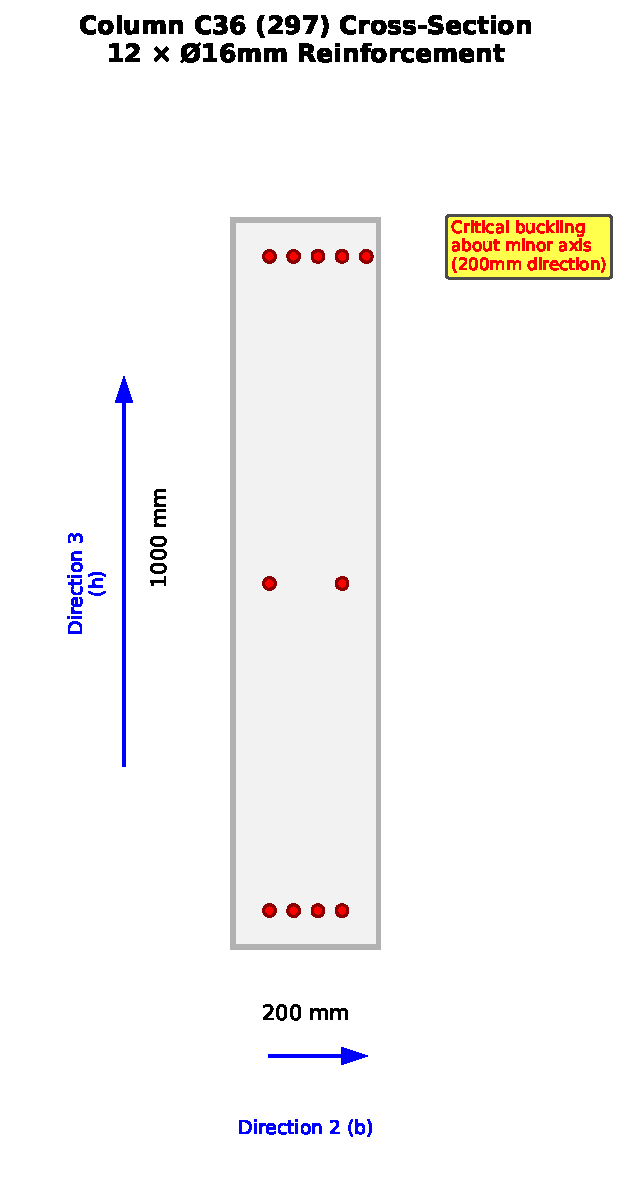
\includegraphics[width=\columnwidth]{column_section.pdf}
\caption{Column cross-section with reinforcement layout}
\label{fig:column_section}
\end{figure}

The column cross-section shows the REBAR_COUNT_PLACEHOLDER × REBAR_SIZE_PLACEHOLDER mm reinforcement arrangement with proper consideration of critical buckling direction.

\section{Design Verification}

\subsection{Strength Interaction}

The column strength is verified using ACI 318-19 interaction diagrams or direct calculation methods. Key parameters:

\begin{table}[h]
\centering
\caption{Strength Verification Summary}
\label{tab:strength}
\begin{tabular}{@{}lcc@{}}
\toprule
\textbf{Parameter} & \textbf{Value} & \textbf{Unit} \\
\midrule
Design Axial Load & PU_PLACEHOLDER & kN \\
Magnified Moment (Method 1) & MC_METHOD1_PLACEHOLDER & kN·m \\
Magnified Moment (Method 2) & MC_METHOD2_PLACEHOLDER & kN·m \\
Steel Ratio, $\rho$ & RHO_PLACEHOLDER & \% \\
\bottomrule
\end{tabular}
\end{table}

\subsection{Compliance Summary}

\begin{table}[h]
\centering
\caption{ACI 318-19 Compliance Verification}
\label{tab:compliance}
\begin{tabular}{@{}lcc@{}}
\toprule
\textbf{Requirement} & \textbf{Status} & \textbf{Reference} \\
\midrule
Slenderness Limits & \textcolor{ghaligreen}{\textbf{OK}} & ACI 6.2.5 \\
Method C Applicability & \textcolor{ghaligreen}{\textbf{OK}} & ACI 6.6.4.4.2 \\
Moment Magnification & \textcolor{ghaligreen}{\textbf{OK}} & ACI 6.6.4.5.2 \\
Strength Interaction & \textcolor{ghaligreen}{\textbf{OK}} & ACI 22.4 \\
\bottomrule
\end{tabular}
\end{table}

\section{Conclusion}

The ACI 318-19 Method C analysis demonstrates that Column COLUMN_ID_PLACEHOLDER satisfies all applicable code requirements for slenderness and stability. The moment magnification approach provides adequate safety factors while maintaining structural efficiency.

\paragraph{Key Design Features}
\begin{itemize}
\item Critical buckling direction properly identified (minor axis)
\item Method C applicability verified ($P_u < 0.75P_c$)
\item Conservative and refined stiffness approaches compared
\item Complete ACI 318-19 Section 6.6 compliance
\end{itemize}

\paragraph{Design Recommendations}
Based on the analysis, the column design is adequate for the applied loads with appropriate consideration of slenderness effects per ACI 318-19 Method C requirements.

% Professional signature block (academic style)
\begin{table}[h]
\centering
\caption*{Professional Certification}
\begin{tabular}{@{}cc@{}}
\toprule
\textbf{Prepared By} & \textbf{Reviewed By} \\
\midrule
Ahmed Ghali, P.E. & Senior Engineer, P.E. \\
Professional Engineer & Professional Engineer \\
Date: \today & Date: \_\_\_\_\_\_\_\_\_\_\_\_\_ \\
\bottomrule
\end{tabular}
\end{table}

% Bibliography section (Cambridge style)
\section*{References}

\begin{thebibliography}{9}
\bibitem{aci318}
ACI Committee 318. (2019). \textit{Building Code Requirements for Structural Concrete (ACI 318-19) and Commentary}. American Concrete Institute, Farmington Hills, MI.

\bibitem{macgregor}
MacGregor, J.G., \& Wight, J.K. (2016). \textit{Reinforced Concrete: Mechanics and Design}. Pearson Education.

\bibitem{nilson}
Nilson, A.H., Darwin, D., \& Dolan, C.W. (2015). \textit{Design of Concrete Structures}. McGraw-Hill Education.

\bibitem{salmon}
Salmon, C.G., Wang, C.K., \& Pincheira, J.A. (2011). \textit{Reinforced Concrete Design}. John Wiley \& Sons.
\end{thebibliography}

\vspace{0.3cm}
{\scriptsize\textcolor{ghaligray}{
This calculation follows ACI 318-19 Method C requirements and professional engineering standards. All calculations and results are subject to independent review and verification per professional engineering protocols.
}}

\end{document} 